\section*{Dati e risultati}

\begin{SCfigure}[0.55][t]
    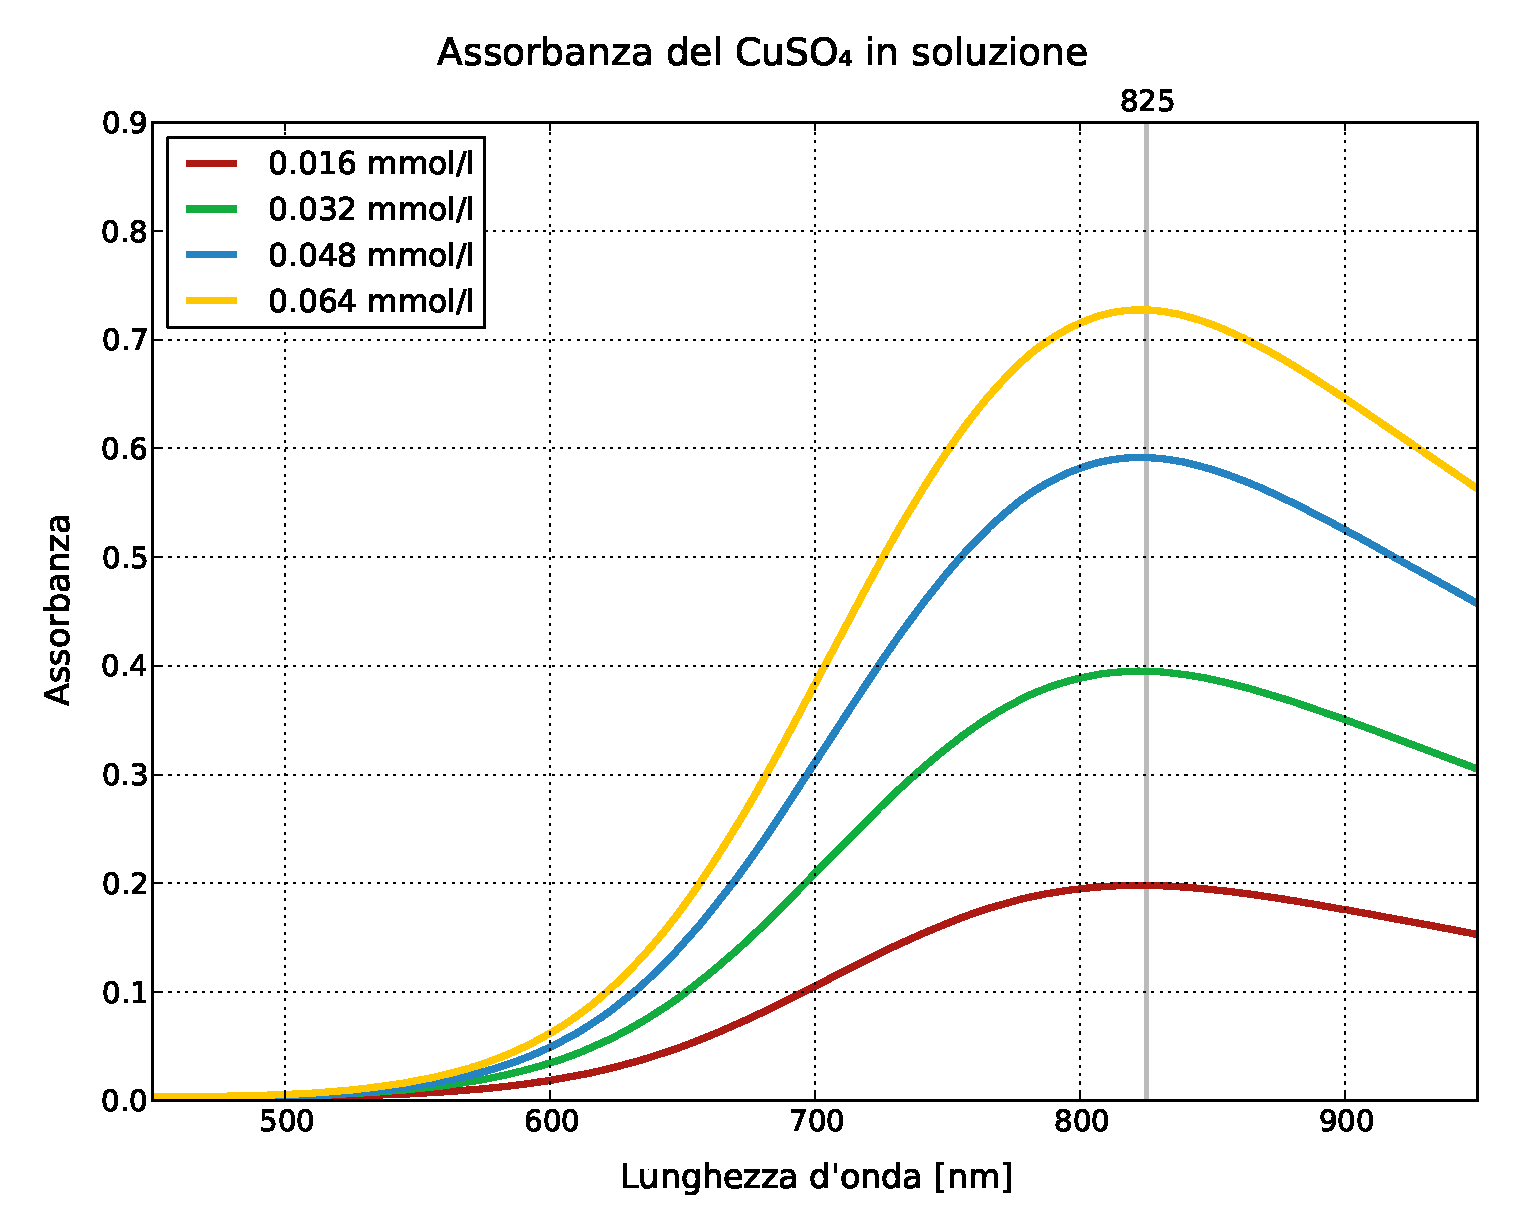
\includegraphics[scale=0.5]{concentrazioni.pdf}
    \caption{Nel grafico sono rappresentate le curve di assorbanza in funzione della lunghezza d'onda delle quattro soluzioni note. \`E stata inoltre evidenziata tramite una linea verticale la lunghezza d'onda di massima assorbanza $\lambda_{max} = \SI{825}{\nano\meter}$.}
    \label{fig:conc}
\end{SCfigure}

Dal grafico in Figura \ref{fig:conc} si può osservare che l'assorbanza delle soluzioni con molarità più bassa è stata predetta con precisione: infatti le soluzioni titolate $\SI{0.016}{\mole\per\litre}$, $\SI{0.032}{\mole\per\litre}$ e $\SI{0.048}{\mole\per\litre} $hanno assorbanza massima a $\lambda_{max}$ relativamente di $0.2$, $0.4$ e $0.6$. La soluzione titolata $\SI{0.064}{\mole\per\litre}$ invece è risultata avere assorbanza massima, sempre in $\lambda_{max}$, di $0.73$. Un valore particolarmente distante dal preventivato $0.8$.

\begin{SCfigure}[0.55][t]
    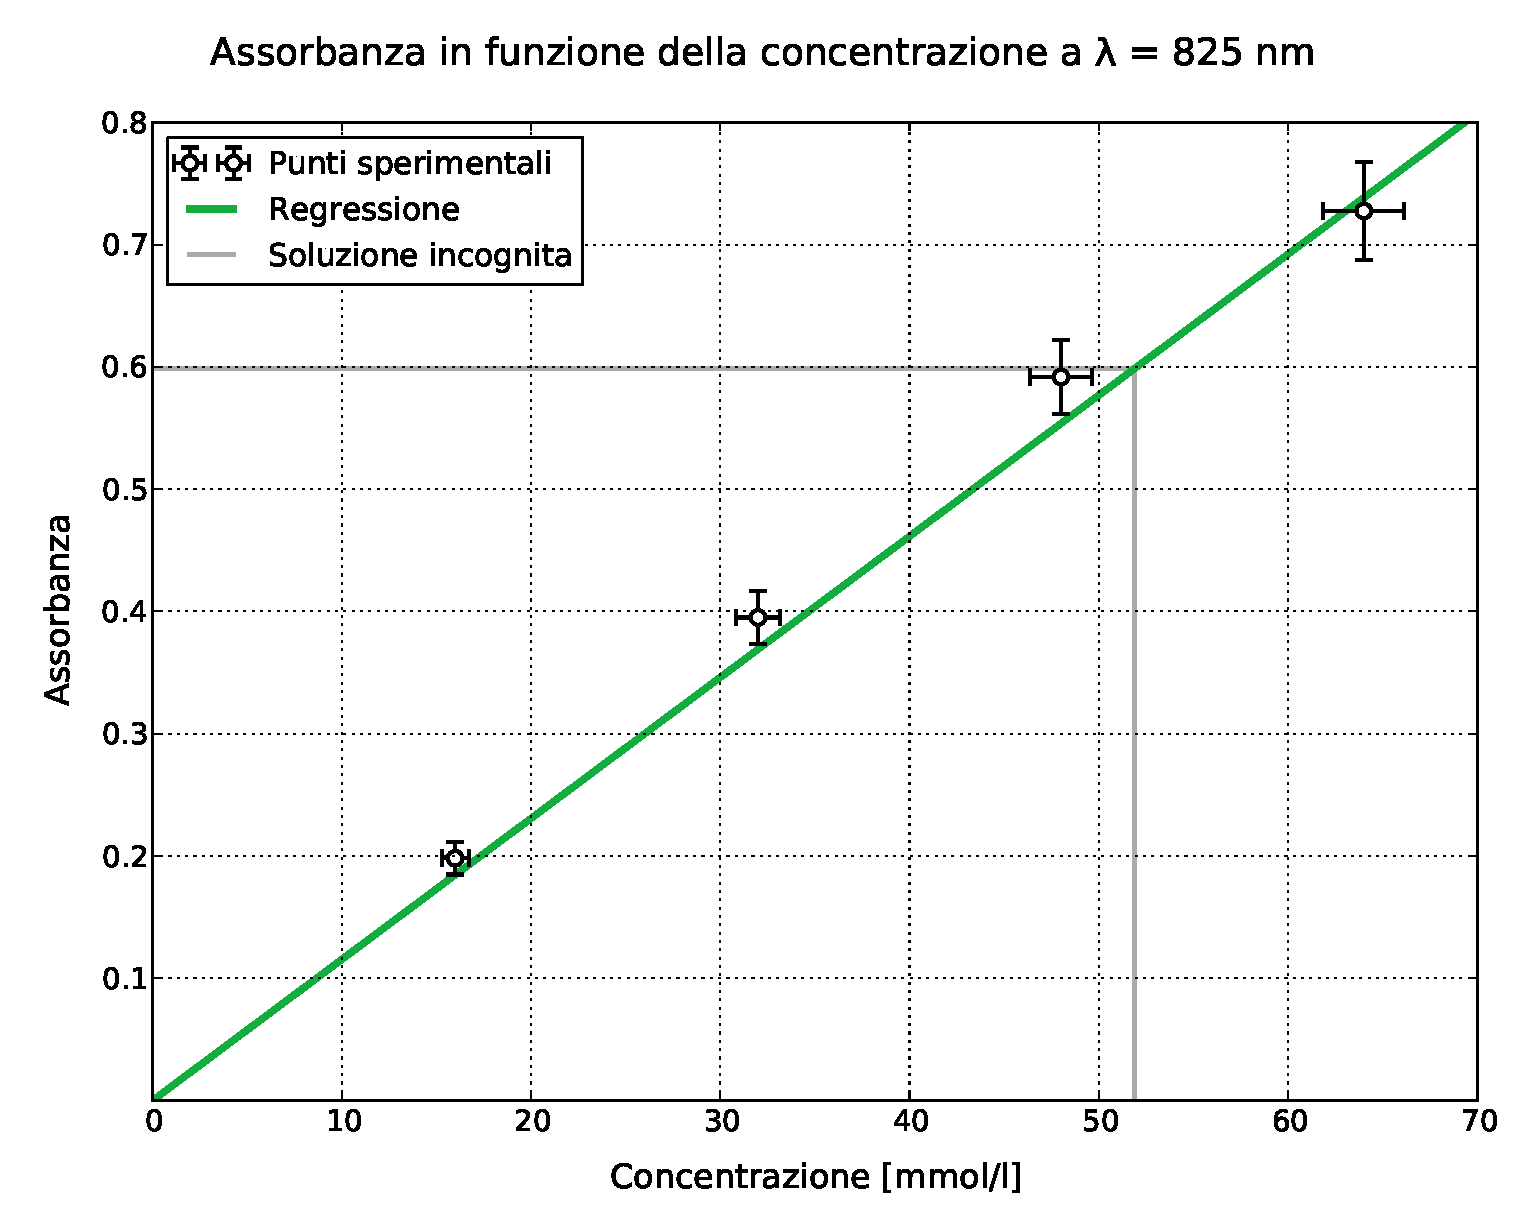
\includegraphics[scale=0.5]{retta.pdf}
    \caption{}
    \label{fig:a_vs_c}
\end{SCfigure}
